\chapter{Gas Species and Smoke}

CFAST simulates a fire as a mass of fuel that burns at a prescribed pyrolysis rate and releases both energy and combustion products.  CFAST calculates species production based on user-defined production yields, and both the pyrolysis rate and the resulting energy and species generation may be limited by the oxygen available for combustion.  When sufficient oxygen is available for combustion, the heat release rate for a constrained fire is the same as for an unconstrained fire.  Mass and species concentrations, assumed to be homogeneous throughout each layer, are tracked by the model as gases flow through openings in a structure to other compartments in the structure or to the outdoors.

The fire chemistry scheme in CFAST is essentially a species balance from user-prescribed 
species yields and the oxygen available for combustion.  Once generated, it is a matter of 
bookkeeping to track the mass of species throughout the various control volumes in a simulated 
building.  It does, however, provide a check of the flow algorithms within the model. 
Since the major species (CO and CO$_2$) are generated only by the fire, the relative accuracy of the 
predicted values throughout multiple rooms of a structure should be comparable. 

\section{Oxygen and CO$_2$}

Gas sampling data are available from a number of the experimental tests.  Figure \ref{fig:Species_Scatter} shows a comparison of predicted and measured values for oxygen and carbon dioxide concentrations, along with a summary of the relative difference for the tests.

\begin{figure}
\begin{center}
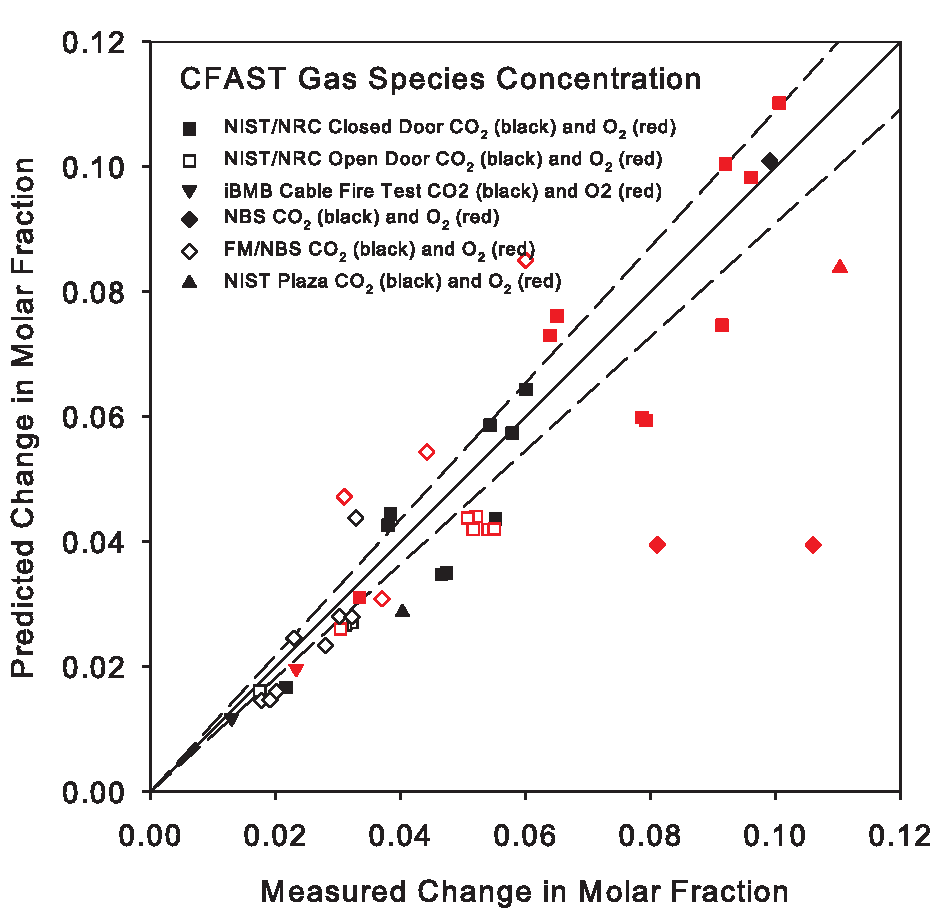
\includegraphics[width=4.0in]{FIGURES/ScatterPlots/Gases}  \\
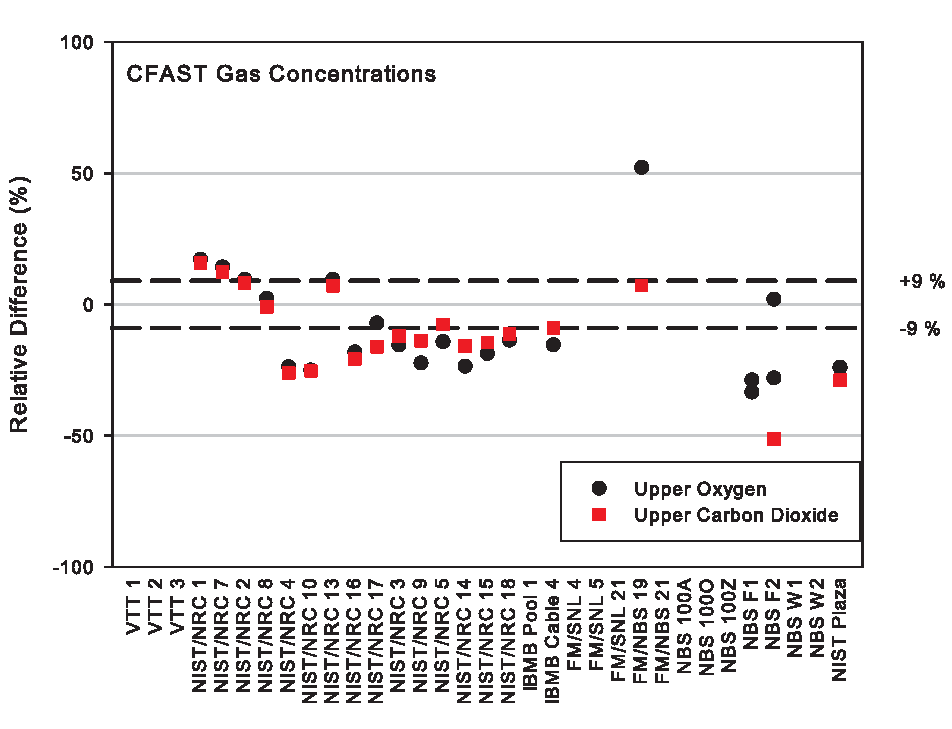
\includegraphics[width=4.0in]{FIGURES/Relative_Diff/Gases}
\end{center}
\caption{Comparison of Measured and Predicted Oxygen Concentration and Carbon Dioxide Concentration.} \label{fig:Species_Scatter}
\end{figure}

CFAST predicts the upper-layer concentrations of oxygen and carbon dioxide within an average of 20~\% of experimental values. Details for individual test series are discussed below. 

\subsubsection{NBS Single Room Tests with Furniture}

For the single-room tests with furniture, the predicted concentrations are lower than those 
measured experimentally (with relative differences of 23 \% for oxygen and 62~\% for carbon dioxide).  This is probably due to the treatment of oxygen limited burning.  In CFAST, the burning rate simply decreases as the oxygen level decreases.  A user prescribed lower limit determines the point below which burning will not take place.  This parameter could be finessed to provide better agreement with the experiment.  For the present comparisons, it was always left at the default value. Since this parameter impacts the overall combustion chemistry in CFAST and the generation of all species, it would impact both oxygen and carbon dioxide.

In addition, species concentrations measured for large fires in small spaces can show considerable spatial variation within the upper layer of the fire compartment \cite{Bundy:2007}. For such under-ventliated fires, the representation of the species concentration in a hot gas layer by a single representative average value may not be valid.

\subsubsection{NIST/NRC Tests}

For the closed-door tests 4 and 10 and open-door Tests 9 and 14, the magnitude of relative difference is higher, under-predicting by 22~\% to 25~\%.  Tests 4, 10, and 16 were closed-door tests with the mechanical ventilation system on.  The higher relative differences for these tests are likely because of a non-uniform gas layer in the experiments with higher oxygen concentration near the mechanical ventilation inlet and lower concentrations remote from the inlet.  In CFAST, the flow from the mechanical ventilation system is assumed to completely mix with the gases in the appropriate gas layer of a compartment.  CFAST consistently under-predicts the drop in oxygen concentration, with Tests 9 and 14 showing a higher relative uncertainty than other closed-door tests.  The cause of a higher-than-average difference is not clear.

\subsubsection{iBMB Cable Fire Test}

CFAST under predicts oxygen and carbon dioxide concentrations by 15~\% and 9~\%, respectively.

\subsubsection{FM Four Room Including Corridor Test Series}

For these four compartment tests, the end of test values of the gas concentrations agree far better than the peak values. With the underlying assumption of all zone fire models of a uniform concentration of gas species throughout a control volume,  it is assumed than the point measurement is the bulk concentration of the entire upper layer.  In reality, some vertical distribution not unlike the temperature profile exists for the gas concentration as well. 

Since this measurement point is near the lower edge of the upper layer for a significant time, it 
should underestimate the bulk concentration until the layer is large in volume and well mixed.  Still, the relative differences for these tests are larger than the NIST/NRC tests, averaging 33~\% for oxygen and 17~\% for carbon dioxide.

\subsubsection{NIST Seven-story Hotel Tests}

For the multiple-story building test, predicted values for CO$_2$, CO, and O$_2$ are lower than 
measured experimentally.  Both the lower burning rate limit as well as leakage in the 100 year- 
old structure probably contributed to the differences between the experiments and model.  In 
addition, values for species yields were simply literature values since no test data were available.

\section{NIST/NRC Test Series, Smoke}

CFAST treats smoke like all other combustion products, with an overall mass balance dependent on interrelated user-specified species yields for major combustion species.  To model smoke movement, the user prescribes the smoke yield relative to the yield of carbon monoxide.  A simple combustion chemistry scheme in the model then determines the smoke particulate concentration in the form of an optical density.  Figure \ref{fig:Smoke_Scatter} shows a comparison of predicted and measured values for smoke concentration along with a summary of the relative difference for the tests.

\begin{figure}
\begin{center}
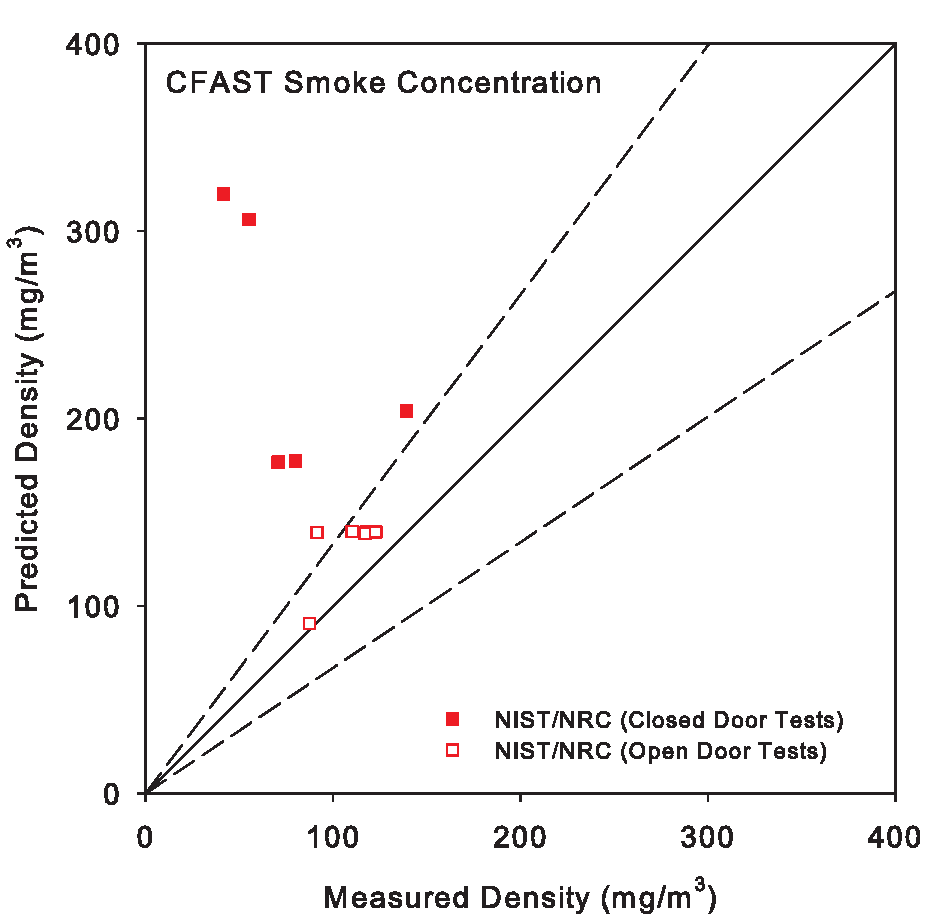
\includegraphics[width=4.0in]{FIGURES/ScatterPlots/Smoke}  \\
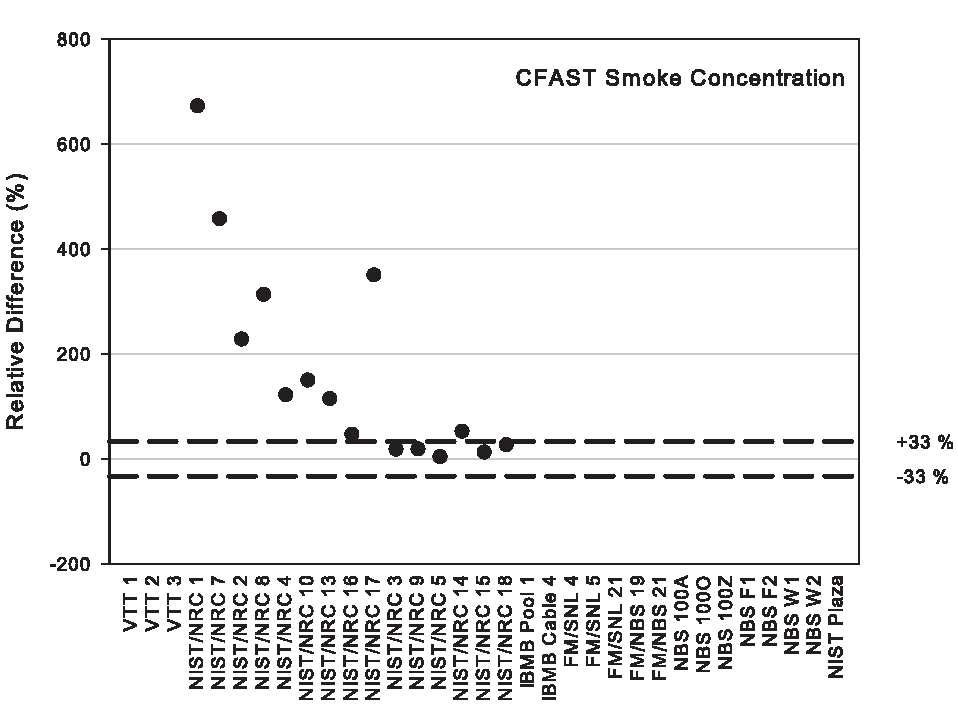
\includegraphics[width=4.0in]{FIGURES/Relative_Diff/Smoke}
\end{center}
\caption{Comparison of Measured and Predicted Smoke Concentration.} \label{fig:Smoke_Scatter}
\end{figure}

Only the NIST/NRC test series has been used to assess predictions of smoke concentration.  For these tests, the smoke yield was specified as one of the test parameters.  There are two obvious trends in the results.  First, the predicted concentrations are within or near experimental uncertainties in the open-door tests.  Second, the predicted concentrations are roughly three to five times the measured concentrations in the closed-door tests.  The experimental uncertainty for these measurements has been estimated to be 33~\%.  The closed-door tests cannot be explained from the experimental uncertainty.

The difference between model and experiment is far more pronounced in the closed-door tests.  Given that the oxygen and carbon dioxide predictions are no worse (and indeed even better) in the closed-door tests, there is reason to believe either that the smoke is not transported with the other exhaust gases or the specified smoke yield, developed from free-burning experiments, is not appropriate for the closed-door tests.  These qualitative differences between the open- and closed-door tests are consistent with the FDS predictions (see reference \cite{NRCNUREG1824_FDS}).

\section{Summary}

Based on the model physics and comparisons of model predictions with experimental measurements, CFAST calculations of oxygen and carbon dioxide concentration are seen as appropriate with the following comments:

\begin{itemize}
\item CFAST uses a simple user-specified combustion chemistry scheme based on a prescribed pyrolysis rate and species yields that is appropriate for the applications studied.
\item CFAST predicts the major gas species close to within 20~\% of experimental measurements.
\item For large fires in small compartments, local species concentration may vary considerably from a bulk average value.  Thus higher uncertainty can be expected for predictions of species concentrations in these scenarios.
\end{itemize}

Use of CFAST calculations of smoke concentration require additional care for the following reasons:

\begin{itemize}
\item CFAST is capable of transporting smoke throughout a compartment, assuming that the production rate is known and its transport properties are comparable to gaseous exhaust products.
\item CFAST typically over-predicts the smoke concentration in all of the NIST/NRC tests, with the exception of Test 17.  Predicted concentrations for open-door tests are within experimental uncertainties, but those for closed-door tests are far higher.  No firm conclusions can be drawn from this single data set.  The measurements in the closed-door experiments are inconsistent with basic conservation of mass arguments, or there is a fundamental change in the combustion process as the fire becomes oxygen-starved.
\end{itemize}